\documentclass{article}

\usepackage{amsmath}
\usepackage{graphicx}
\usepackage{listings}
\graphicspath{ {graphs/} }

\title{2XB3 Lab3}
\author{
  Yi Luo\\
  \texttt{400254211}\\
  \texttt{luoy94@mcmaster.ca}\\
  \texttt{L02}
  \and
  Frank Yang\\
  \texttt{400243777}\\
  \texttt{yangf51@mcmaster.ca}\\
  \texttt{L02}
  \and
  Harrison Chiu\\
  \texttt{400261400}\\
  \texttt{chiuh@mcmaster.ca}\\
  \texttt{L02}
}
\date{\today}

\begin{document}

\maketitle

\begin{abstract}
This paper analyzes different time complexities of quicksort. Specifically it looks into the time complexities of various quicksort implementations, including multiple pivots, different pivots, small lists, and worst case performance. Github Link: https://github.com/frankyang3/2xb3lab3
\end{abstract}

\pagebreak 
\section*{Method}
 The inplace quicksort was a standard implementation, while for the multi-pivot quicksort we chose to select the first \verb|x| elements as pivots, where \verb|x| is the amount of pivots in the sort. The pivots were then sorted based using python's standard sort. The rest of the implementation is similar to the given function \verb|my_quicksort|, a non-inplace version. We conducted tests for these using a separate function, written as \verb|tests|. The program was run as shown below.
 \break
 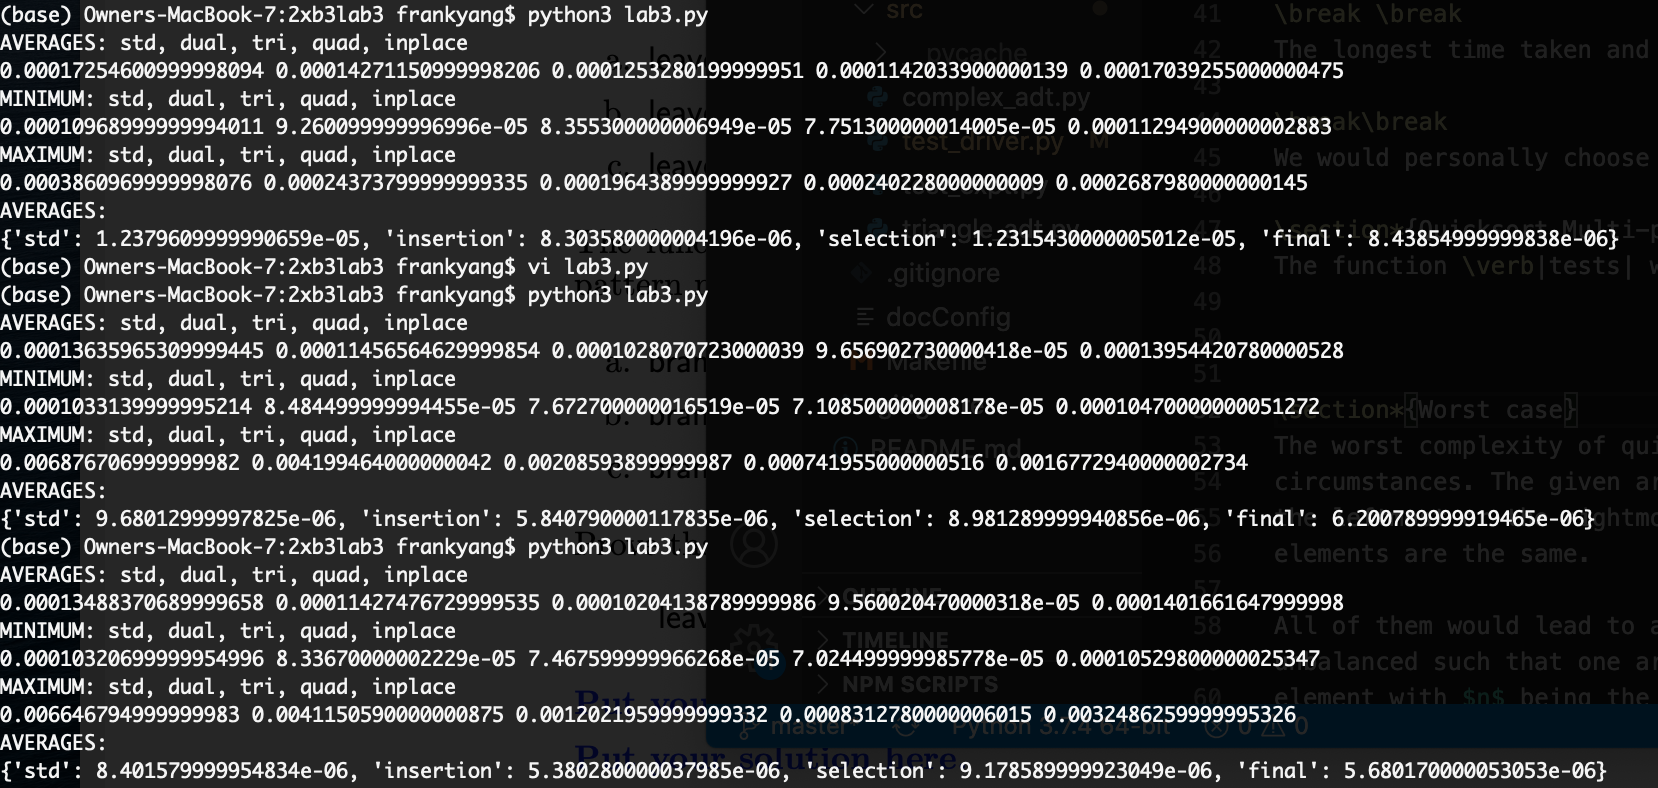
\includegraphics[width=0.8\textwidth]{Lab3Method}
 \break This function essentially loops the call of quicksort using the given \verb|create_random_lists| to generate data sets. Each iteration was timed using \verb|timeit|, and stored into an array. At the end, the maximum, average, and minimum times were calculated and displayed. For the worst case experiment, we first calculated the time complexity for quicksort, as well as the worst case. We then wrote our own bubble sort, insertion sort and selection sort. Using the function \verb|create_near_sorted_list|, we were able to identify which sort performs the best based on how sorted the list given is. This data was collected using \verb|pandas| and published on csv files in the github. Lastly we tested our small list runtimes through a function \verb|small_lists_tests|. This was built similarly to the \verb|tests| function above, but use a list size of 10. Similarly, we iterate the function 1000 times, and obtain the average runtimes for insertion sort, bubble sort, and selection sort. This then printed.

\section*{Quicksort Inplace}
Using the \verb|timeit| package and \verb|create_random_lists|, we wrote a testing function called \verb|tests| This function essentially ran the inplace quicksort and the traditiona \verb|my_quicksort| implementation 100 times using a different random list. Then it would take the average, the maximum, and the minimum runtimes. It was found that the average runtimes for both were identical, over 10000 iterations, it was about 0.00013s to sort each.
\break \break
The longest time taken and the least time taken were more volatile as expected, and showed differences in runtime. Upon running the tests to 10000 iterations, it was found that the \verb|inplace| implementation consistently took less maximum time. Although we did not prove this mathematically, this is a strong indicator it has a better worst case runtime. Interestingly, the least amount of time taken, or best case scenario was quite consistent across both implementations, at around 0.0001s to sort. As none of these are extreme outliers, the runtime for both implementations is effectively the same.

We would personally choose to use the inplace implementation for a better worst case scenario, resulting in more consistent runtimes in a wider range of scenarios. However, it should be noted that the correct quicksort implementation should obviously be chosen depending on the situation, as both implementations have their own merits.

\section*{Quicksort Multi-pivot}
The function \verb|tests| was used once again to run each sort 10000 times with a random list. Each test is similarly generated with \verb|create_random_lists| and timed with \verb|timeit|. Our results showed the average runtime for each quicksort  to be: 0.00013s for one pivot, 0.00011s for two pivots, 0.00010s for three pivots, and 0.00009s for 4 pivots. This clearly shows that the 4 pivots is the fastest on average. With our program, we were also able to gather the fastest and slowest times over the 10000 trials, and while numbers differ due to obvious reasons of variance, the trend stayed the same. Four pivots consistently had faster times than three pivots, which had faster times than two, with one pivot being the slowest. Because of this, we recommended using the 4 pivot quicksort, as it has the fastest runtime. It should be noted, however the more pivots there are, the more complicated choosing and placing the pivots becomes. This means that it would not be the most efficient to just create as many points as possible, there must be a optimal point for a data set of a certain size. Within the scope of our experiment however, four pivots performs the best overall.



\section*{Worst case}
The worst complexity of quicksort is $n^2$. It happens under the following 
circumstances. The given array is already sorted or reversely sorted with 
the leftmost or the rightmost element chosen as the pivot. The given array’s 
elements are the same.

All of them would lead to a situation where the divided arrays are totally 
unbalanced such that one array has only one element while the other has $n - 1$ 
element with $n$ being the size of the parental array. As a result, the time 
complexity would be as such:
\begin{equation*}
n + (n - 1) + (n - 2) + (n - 3) + … + 2 = n * (n + 1) / 2 – 1 = \Theta{n^2}
\end{equation*}

A graph is attached showing the average case performance vs the worst case performance vs n.

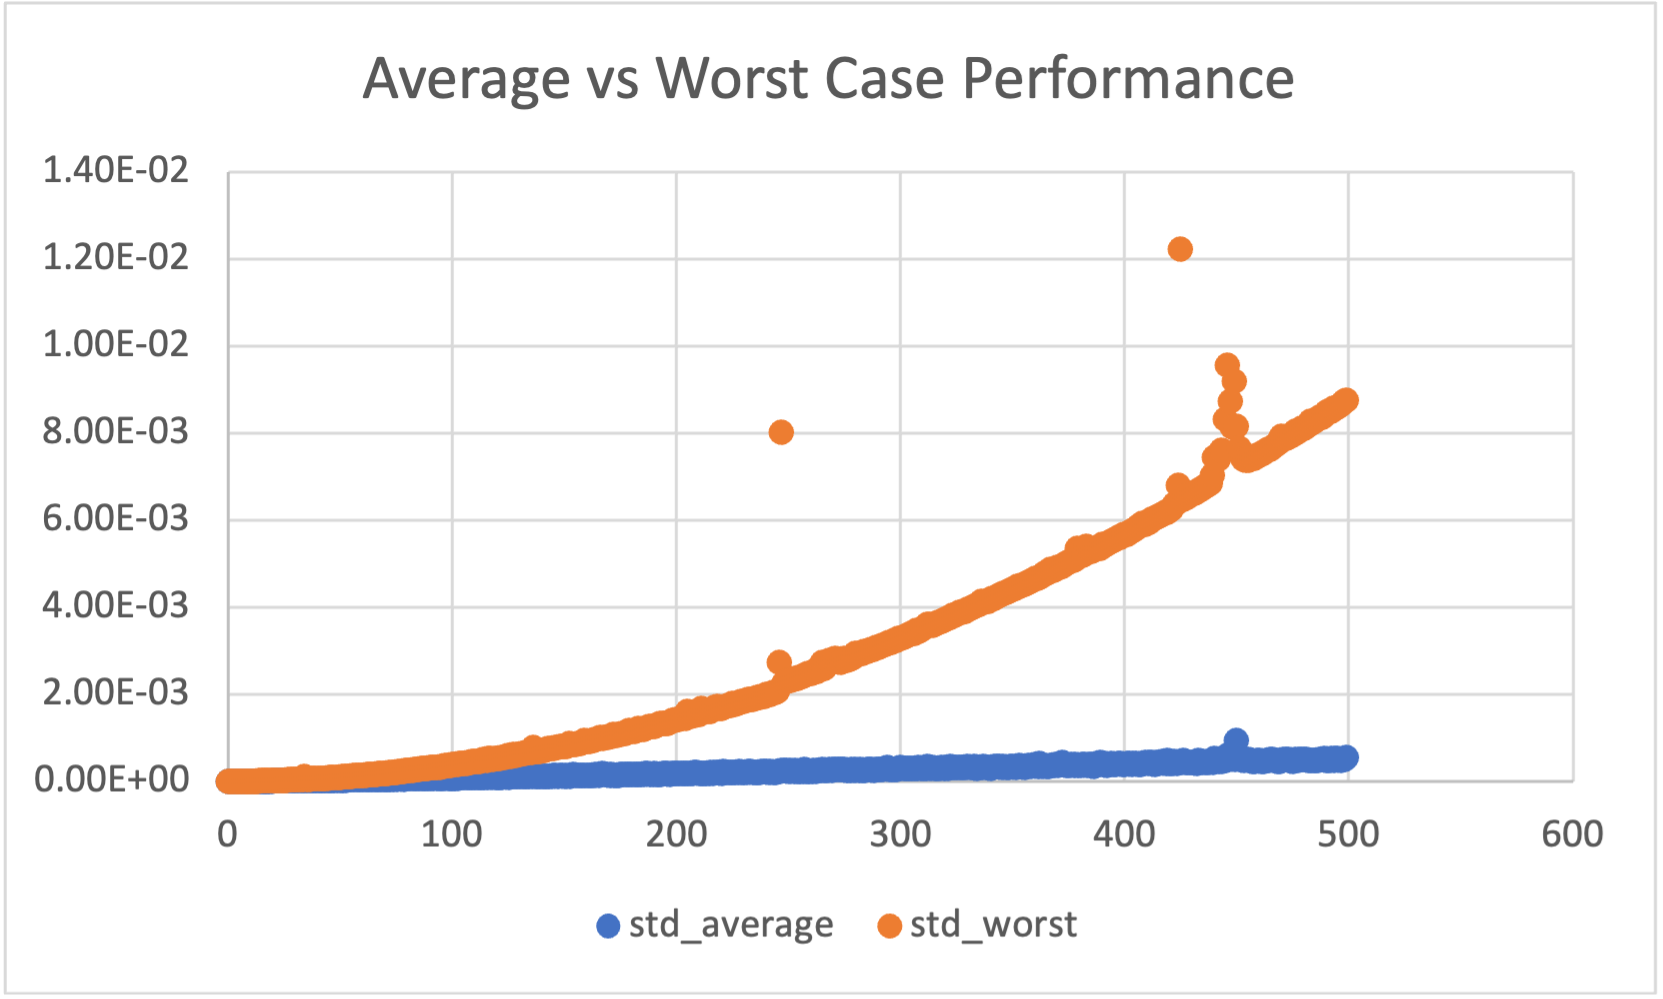
\includegraphics[width=0.8\textwidth]{average_vs_worst_case_performance}

\medskip
The function \verb|create_near_sorted_list| creates near-sorted-list based off 
some input factor. The lower the factor, the closer to being sorted the created list is.

Bubble sort will out-perform quicksort when a given list is close to being sorted 
since it only takes one or few iterations for the bubble sort to terminate, yielding 
a linear complexity($\Theta{n}$). Attached is a graph comparing their performance 
with factor ranging from 0 to 0.99. Note that the lists sorted are of length 996 
instead of 1000 as specified since it would otherwise generate \verb|RecursionError|.

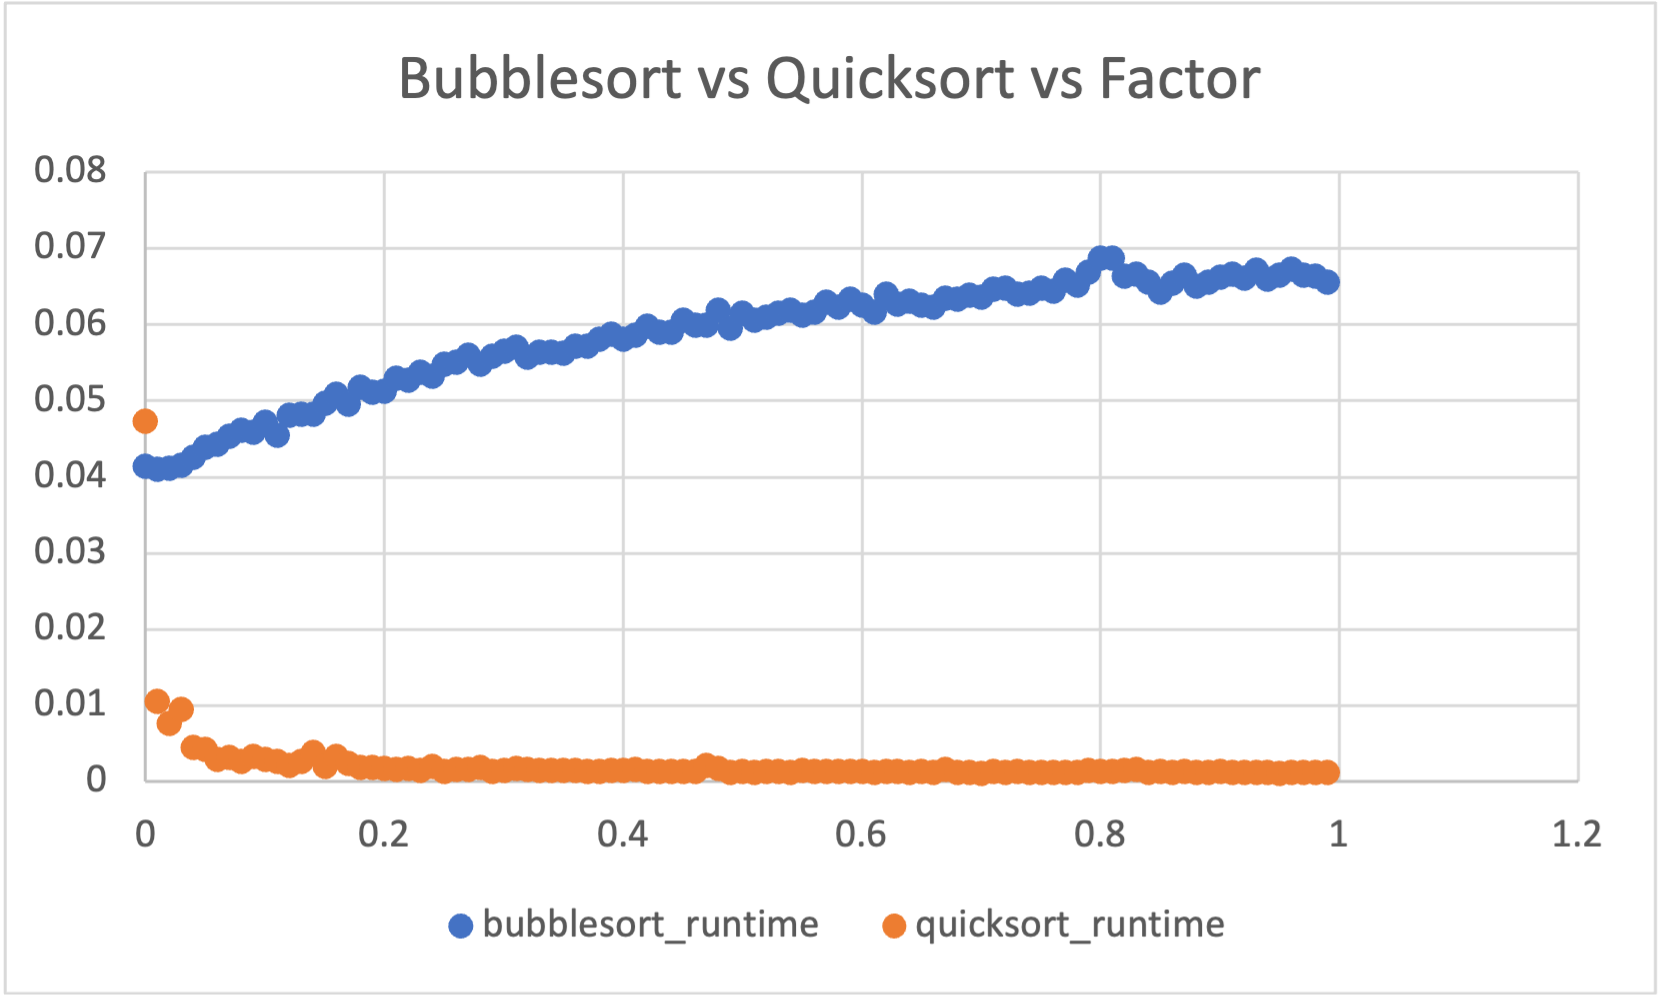
\includegraphics[width=0.8\textwidth]{bubblesort_vs_quicksort_vs_factor}

Bubble sort out-performs only when factor is extremely close to zero.

\medskip
Selection sort always has a complexity of $n^2$. Attached is a graph comparing their 
performance with factor ranging from 0 to 0.99. Note that the lists sorted are of 
length 996 instead of 1000 as specified since it would otherwise generate \verb|RecursionError|.

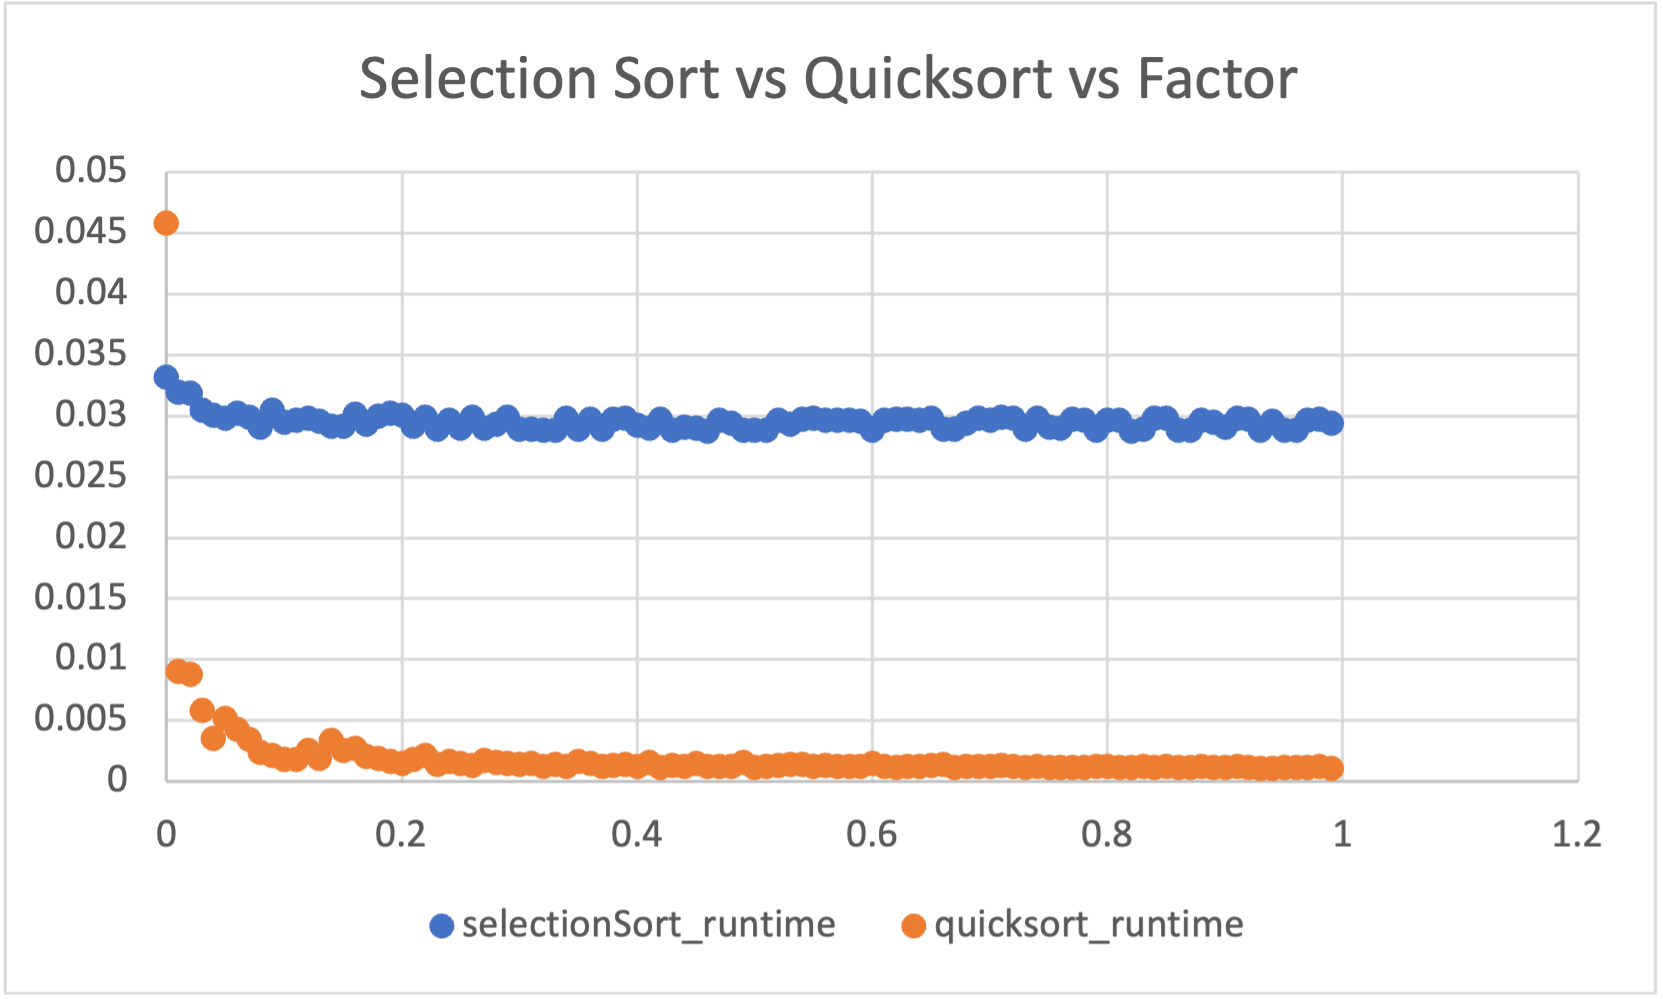
\includegraphics[width=0.8\textwidth]{selectionSort_vs_quicksort_vs_factor}

Selection sort out-performs only when factor is extremely close to zero.

\medskip
Insertion sort will out-perform quicksort when a given list is close to being sorted, 
yielding a linear complexity($\Theta{n}$). Attached is a graph comparing their 
performance with factor ranging from 0 to 0.99. Note that the lists sorted are of 
length 996 instead of 1000 as specified since it would otherwise generate \verb|RecursionError|.

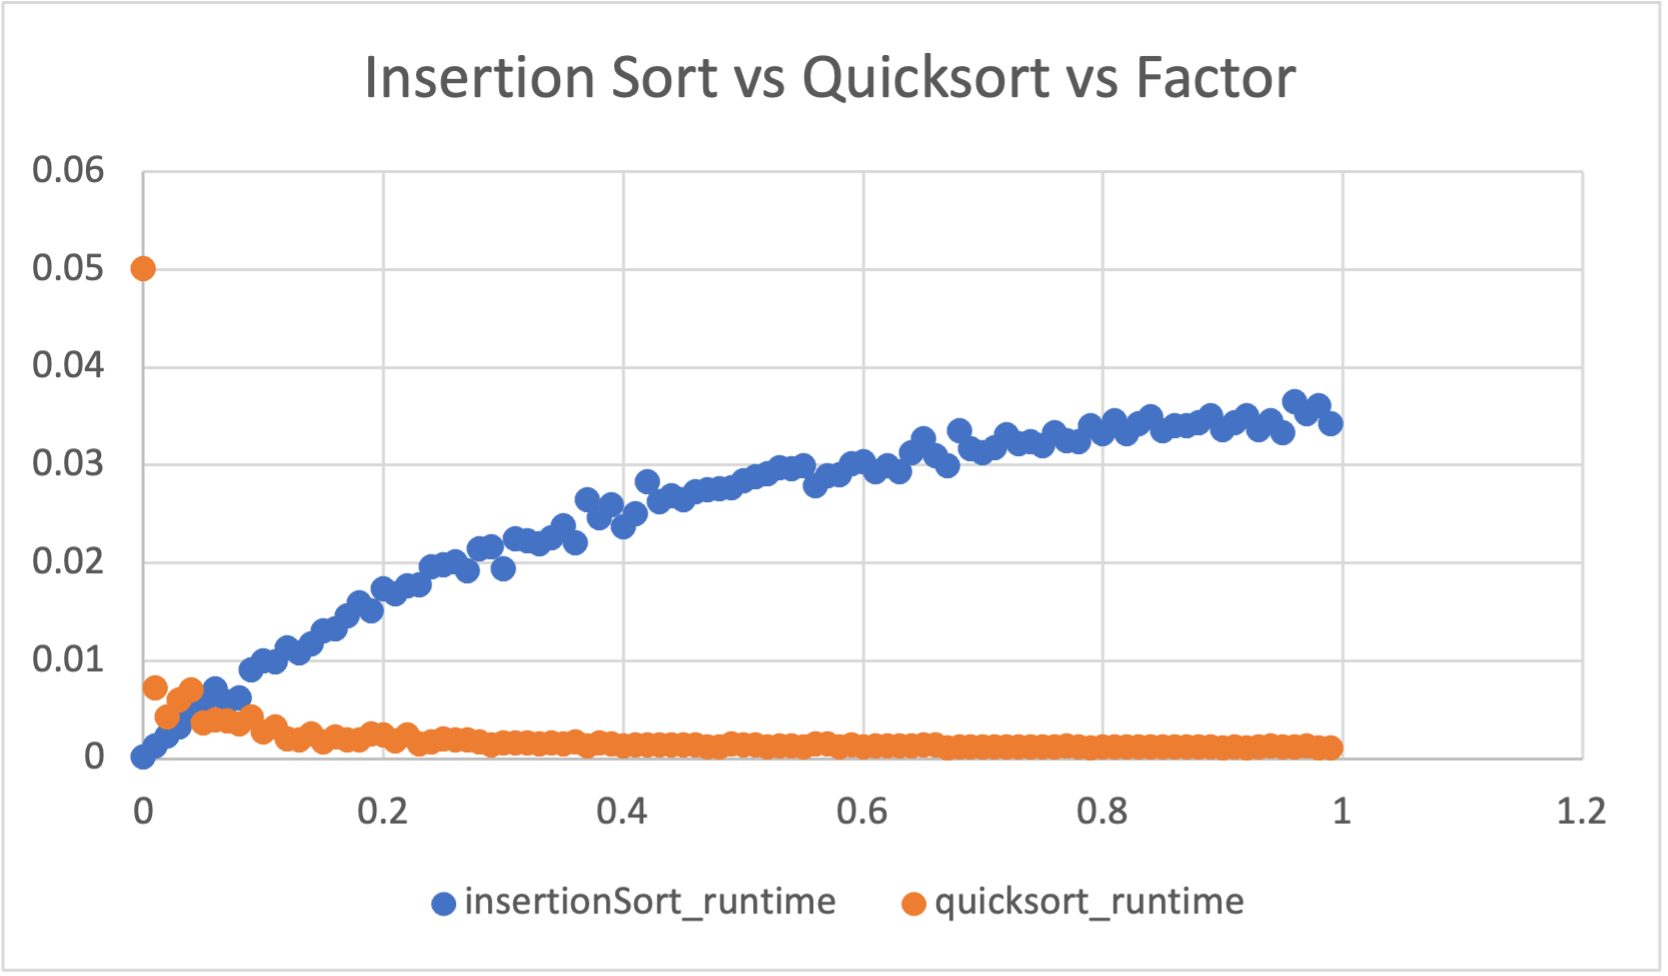
\includegraphics[width=0.8\textwidth]{insertionSort_vs_quicksort_vs_factor}

Insertion sort out-performs when factor approximately is smaller than 0.05.

\section*{Small lists}
For small lists (small values of $n$), elementary sorting algorithms’ time complexity is measured. Selection and insertion sorts’ running time were tested. The results were (also seen in the graph but these are the averages for values of $N < 50$) \verb|{'std': 9.19201014767168e-06, 'insertion': 5.821419908897951e-06,|\break \verb| 'selection': 9.893930109683424e-06, 'final': 6.013410202285741e-06}| (std is the \verb|my_quicksort|) where the value of the dictionary is the average over 100 trials of running the function in seconds. It is clear that the standard quicksort is very slow compared to insertion and our final sort for small values of $n$ even though they have $O(n^2)$ time complexity compared to quicksort’s time complexity of $O(nlog(n))$. The difference is approximately $4e-6$ between \verb|std| and \verb|insertion|. This is likely because for small values of $n$, quicksort requires more memory from its recursive calls and insertion sort requires few swaps and comparison for small arrays. Furthermore, $O(n)$ is a measure of its running time for large values of $n$ which ignores all constant factors. Only for large values of $n$ do the constant factors such as $+c$ are ignored because the growth of the function, $O(n)$, dominates all other factors. Selection sort is quite slow at $9.89e-6$. This is expected; its running time is always $O(n^2)$. This is because no matter the ordering of the array, selection sort will traverse through the array approximately $\frac{N^2}{2}$ times to find the minimum $N$ times. 

The graph also shows that for small values of $N < 200$, insertion sort has smaller runtimes than the other algorithms. However, this changes as $N$ becomes much larger and its runtimes become the expected value from its big-O values. To conclude our most notable observations, insertion sort is faster than quicksort for small values of $n$ and can be used to improve our quicksort.

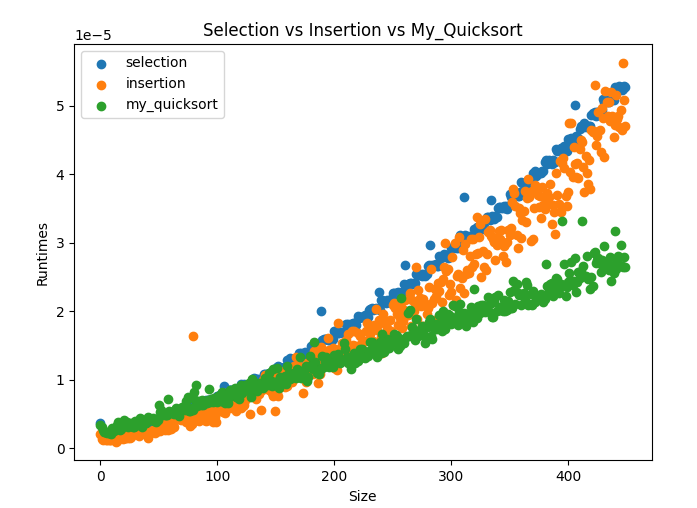
\includegraphics[width=0.8\textwidth]{elementarySortsComparisons}

Our implementation of an improved quicksort is a hybrid of insertion sort and quicksort. From our observations, insertion sort has a lower running time than quicksort for small values of $n$. Our main goals were to improve the standard quicksort given in \verb|my_quicksort()| both in terms of time and space complexity. Using this to our advantage, we can switch between quicksort and insertion sort to use both of them during their ideal conditions. It will still mainly use quicksort because for large values of $n$, it is still much faster than insertion sort ($O(nlog(n))$ < $O(n^2)$ for large $n$). However, for small values of $n$ (we arbitrarily chose 10 as the small value), the sorting algorithm will switch to insertion sort. When the array has reached the condition to start the insertion sort, it will have already been partly sorted. Insertion sort is very quick for partly sorted arrays because it will need to do less comparisons, and therefore, less swaps. Its running time in this case (small array and partly sorted) will be close to $O(kn)$ for some $1 \geq k$. Furthermore, the quicksort algorithm does not follow the style of \verb|my_quicksort| because it requires more space when it physically creates new subarrays to recursively sort them; it has a smaller space complexity. Since the sorting algorithm now stops its recursion when its subarray is approximately 10,  its recursion depth is significantly lower. 

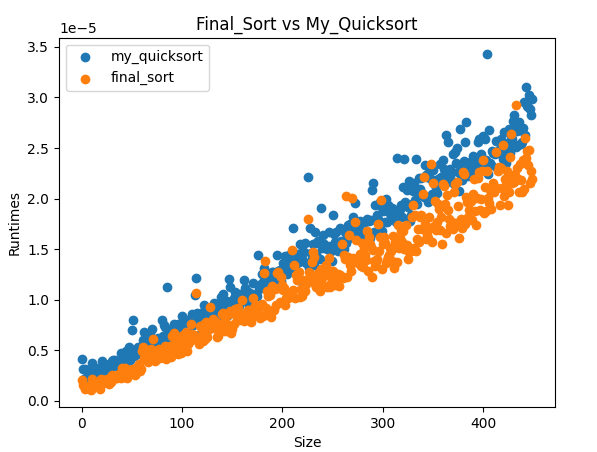
\includegraphics[width=0.8\textwidth]{quicksortFinalSort}

The worst case of this algorithm is a reverse sorted list. It is the worst case for both quicksort and insertion sort (which our algorithm uses). For quicksort, it causes the partition to be very unbalanced because every number will be less than or equal to it (if we choose the first number as our pivot number). This will also maximize the recursive depth to a size of nearly $N-1$. Furthermore, the final subarrays in which insertion sort runs will also be reverse sorted and so, it will have a maximum runtime of $10^2$ (we arbitrarily chose 10 as the breaking point for insertion sort to run). Since both of these sorting algorithms are $N^2$ in the worst case, our algorithm is also $N^2$ as seen in the graph. It has a similar shape to $N^2$.

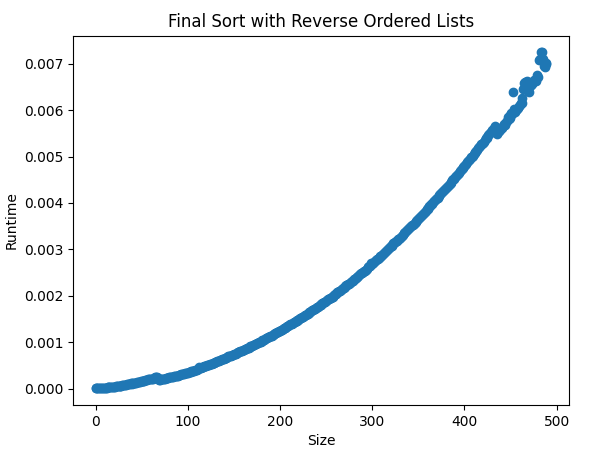
\includegraphics[width=0.8\textwidth]{finalSortReverseOrderedLists}

Since our sorting algorithm is still predominantly quicksort and still mostly uses quicksort to sort, the best case will still depend on quicksort’s best case. Insertion sort is only used for very small lists, its time complexity is negligible. Its best case is when the pivot number is exactly in the middle such that it partitions the numbers evenly. An example is when the array is randomly ordered because a random pivot will be approximately in the middle. This also minimizes the recursive depth (and thus the memory usage) to $\log_2 N$ (height of the binary tree). Quicksort will have a best case time complexity of $O(N\log N + c)$ or $O(N\log N)$ where $c$ is some constant from insertion sort’s time complexity. As seen in the graph, the running times increase somewhat linearly with a small curve at the beginning, similar to $O(N\log N)$.

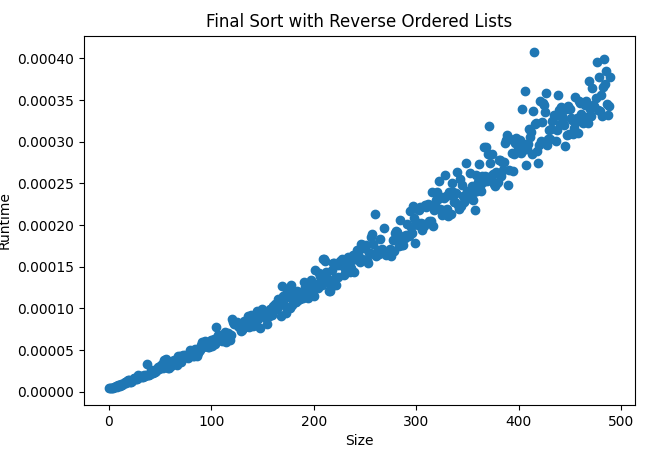
\includegraphics[width=0.8\textwidth]{finalSortRandomLists}

In the average case, the finalsort will be the same as quicksort. As explained before, finalsort is still predominantly quicksort and thus the average case will depend on it. The average case is when the subarrays are partitioned approximately equally (as seen in the graph below). This is because it is very likely for a randomly chosen pivot to be in the middle 50\% of the numbers. Thus, the average case for finalsort is $O(N\log N)$.

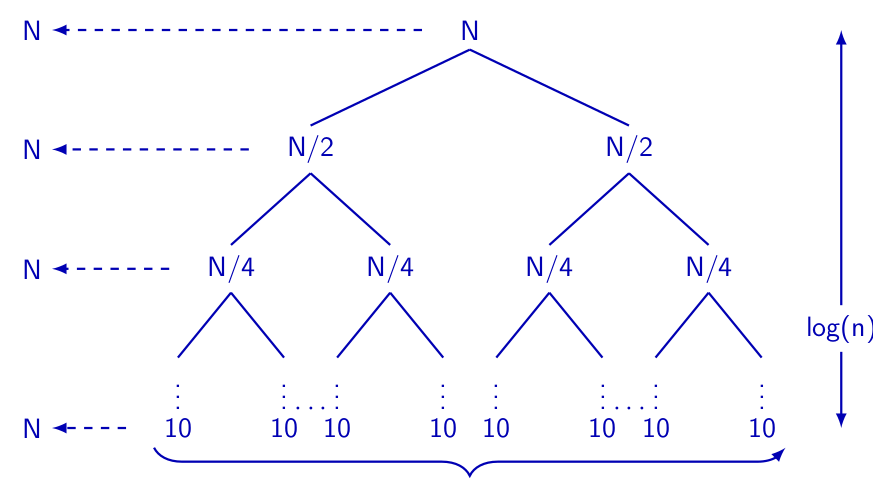
\includegraphics[width=0.8\textwidth]{bestCase}\\
The values in this graph are approximate for the average case and exact for the best case. The height of the recursion tree is slightly less than the shown $\log(N)$, but since the finalsort does mostly quicksort, it is still approximately $\log(N)$. This graph also visually shows the reason why the best case's (and average case's) recursion depth (explained before) is approximately $\log(N)$ and why the total time complexity is approximately $N\log(N)$. Each level does $N$ amount of work with approximately $\log(N)$ levels in the tree.


\section*{Sources of Error}
Our experiment most likely does not contain any sources of error. The one source of error may be a bug in computer running, causing the runtime of an iteration to be higher than it actually is, or a statistical anomaly where the generated lists are always unfavourable to a certain implementation. As both of these are statistically impossible due to the sample size of three computers and more than 40,000 iterations, we believe the conclusions drawn from the experiment to be accurate.

\section*{Conclusion}
In conclusion, this experiment tested the runtimes of different sorting algorithms. Specifically, it tested the runtime of the inplace implmentation of quicksort vs a standard one, Quicksort with multiple pivots, and quicksort vs. bubble sort, insertion sort, and selection sort, testing both worst case and small lists of size 10. It was found that inplace and standard implementations performed similarly on average, quicksort with more pivots generally performs better than with less pivots, and quicksort is outperformed by bubble sort, insertion sort, and selection sort when the list is close to sorted. Lastly, it was found that for small lists, quicksort is similarly outperformed, but drastically outperforms the other sorting algorithms in larger lists.

\end{document}
